\documentclass[12pt]{beamer}
\usetheme{metropolis}
\definecolor{myblue}{RGB}{34, 70, 135}
\setbeamercolor{frametitle}{fg=white}
\usepackage{listings}
\lstset{
  basicstyle=\ttfamily\small,
  keywordstyle=\color{myblue}\bfseries,
  commentstyle=\color{gray},
  stringstyle=\color{orange},
  showstringspaces=false,
  frame=lines,
  columns=fullflexible,
}
\usepackage{tikz}
\usetikzlibrary{shadows}
\begin{document}
% Stunning Title Slide
{
\begin{frame}[plain]
  \vfill
  \centering
  {\usebeamerfont{title}\usebeamercolor[fg]{title}\Huge \textbf{Image Generation}\par}
  \vskip1em
  {\usebeamerfont{subtitle}\large Face Generation using Deep Generative Models \LaTeX\par}
  \vskip2em
  {\usebeamerfont{author}\large Nikos Nteits\par}

  \vskip2em
  {\usebeamerfont{date}\normalsize \today\par}
  \vfill


\end{frame}










\begin{frame}{Outline}

In this Project  Generative models will be developed from scratch and their performance will be compaired. Main objective is to tune a Variational autoencoder and a Deep Convolutional GAN, models notorious for their training instability. Image generation was picked as results are easier to interpret and score. 
\end{frame}



\begin{frame}{Dataset}
The Dataset that was used was the CelebA dataset of Kaggle. The dataset contains 202,599  face images of various celebrities with a suplementary feature vector of legth 40.

\end{frame}



\begin{frame}{Sample:}
Dataset constists of 128x128 images. A sample :
\begin{center}
    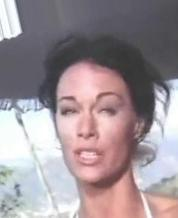
\includegraphics[width=0.5\linewidth]{000233.jpg}
    
    % Example legend below the image
    \vspace{1em}
    \begin{tabular}{ll}
      \textcolor{black}{ Figure 1 }\\

      % Add more as needed
    \end{tabular}
\end{center}
\end{frame}


\begin{frame}{cVAE:}
At first a conditional Variational Autoencoder with 4 convolutional blocks for the image and a shallow feedforward part for the features was used. A latent dimention of 200 was chosen and MSE + KL divergence as Loss. Results were blurry, something usual for VAE . Further tests will be performed with non symmetrical  encoder-decoder schema and with the use of skip connections.
\end{frame}

\begin{frame}{DCGAN:}
A DCGAN was used to generate images from the images in the celeba dataset. Generator and Discriminator consist of 4 convolutional blocks. Images were a crispier compaired to the cVAE. Many of them were similar, so a problem of mode collapse is probably present. Further testing will be held with empowerment of the generator and the use of Wasserstein distance.
\end{frame}

\end{document}